\documentclass[twocolumn,trackchanges]{aastex6}

\usepackage{amssymb,amsmath}

\newcommand{\halpha}{H$\alpha$}
\newcommand{\nh}{$N_{\rm H}$}

\received{}
\revised{}
\accepted{}
\published{}
%\submitjournal{\textit{The Astrophysical Journal Letters}}

\shorttitle{} 
\shortauthors{Shimizu T. T. \emph{et\,al.}}

\begin{document}

\title{Obscuration in Seyfert 1.9 Active Galactic Nuclei}
%\author[0000-0002-2125-4670]{T. Taro Shimizu}
\author{T. Taro Shimizu and Richard I. Davies}
\affiliation{Max-Planck-Institut f\"{u}r extraterrestrische Physik, Postfach 1312, 85741, Garching, Germany}
%\author{Richard I. Davies}
%\affiliation{Max-Planck-Institut f\"{u}r extraterrestrische Physik, Postfach 1312, 85741, Garching, Germany}
\author{BASS Collaboration}
\affiliation{Everywhere}
%\correspondingauthor{T. Taro Shimizu}
\email{shimizu@mpe.mpg.de}

\begin{abstract}
\end{abstract}

\keywords{galaxies: active -- galaxies: nuclei -- galaxies: Seyfert}

\section{Introduction}\label{sec:intro}
\section{Sample and Data}\label{sec:data}
Our parent sample consists of all AGN in the BAT AGN Spectroscopic Survey (BASS; Koss et al. in preparation). BASS analysed both new and archival optical spectra for a large fraction of the AGN detected as part of the 70-month \textit{Swift} Burst Alert Telescope (BAT) \citep{Gehrels:2004qf, Barthelmy:2005ul} catalogue \citep{Baumgartner:2013fq}. \textit{Swift}/BAT has been continuously surveying the entire sky at high energies (14--195 keV) that allows for nearly complete samples of AGN up to the Compton thick limit ($N_{\rm H} < 10^{24}$ cm$^{-2}$) and reduces selection effects associated with host galaxy contamination and obscuration.

For this work, we need reliable measurements of the broad \halpha{} flux, intrinsic hard X-ray flux, and X-ray absorbing column density. Therefore, we chose all AGN with detected broad \halpha{} from the original BASS analysis as well as AGN that were part of the BASS X-ray spectral analysis presented in Ricci et al 2017, submitted. The key measurements obtained from the X-ray spectral analysis are \nh{} estimates and absorption corrected 14--150 keV flux (hereafter referred to as the intrinsic X-ray flux). 

Broad \halpha{} and intrinsic X-ray fluxes were converted to luminosities using either the redshift independent distances compiled from the NASA/IPAC Extragalactic Database\footnote{\url{http://ned.ipac.caltech.edu/}} or luminosity distances calculated based on the measured redshifts from the spectral analysis and our chosen cosmology ($H_{0}=70$ km s$^{-1}$ Mpc$^{-1}$, $\Omega_{m} = 0.3$).

We limited our sample based on the following requirements:
\begin{enumerate}\itemsep1pt
\item Seyfert classification of 1, 1.2, 1.5, 1.8, or 1.9 according to \citet{Winkler:1992kx}
\item X-ray flux and \nh{} measurement
\item Reliable distance measurement
\item Quality flag of 1 or 2 for the spectral fitting of the \halpha{} region.
\end{enumerate}

This last requirement ensured we removed all sources whose spectra either did not cover the \halpha{} spectral region or the spectral fitting were unreliable. For a detailed description of the optical spectral fitting and explanation of each flag, see the BASS Data Release 1 publication (Koss et al. 2017; submitted). 

Our final sample contains 218 AGN with 22, 67, 68, and 61 Sy 1s, 1.2s, 1.5s, and 1.9s respectively. The BASS sample does not contain any Sy 1.8s 
 
\section{Results}\label{sec:results}

\subsection{\nh{} Distribution}
We first start by showing the \nh{} distribution for the whole sample in Fig.~\ref{fig:nh_dist} regardless of whether the source has a broad \halpha{} measurement. While there is an increase in the number of X-ray absorbed AGN moving from Sy 1s to 1.9s, the biggest increase certainly occurs for the Sy 1.9 subsample. If we arbitrarily create a cutoff at \nh$=10^{22}$ cm$^{-2}$ for X-ray unabsorbed and absorbed AGN, the fraction of X-ray absorbed AGN is 0, 0.07, 0.07, and 0.53 for Sy 1s, 1.2s, 1.5s, and 1.9s respectively. For reference, the fraction of Sy 2s that are X-ray absorbed is 0.94. Therefore, the level of X-ray absorption in Sy 1.9s seems to be intermediate between Sy 1-1.5s and Sy 2s based on the fraction of sources with high X-ray absorption

If the same structure within AGN (i.e. dusty torus) causes both optical obscuration and X-ray absorption then we would expect to observe a level of optical obscuration in Sy 1.9s consistent with the X-ray \nh{} measurements. To measure the optical obscuration in our objects, we use the observed broad \halpha{} luminosity.

%%%%%%%%%%%%%%%%%%%%FIGURE: NH Distribution%%%%%%%%%%%%%%%%%%%%%%%%%%%
\begin{figure}
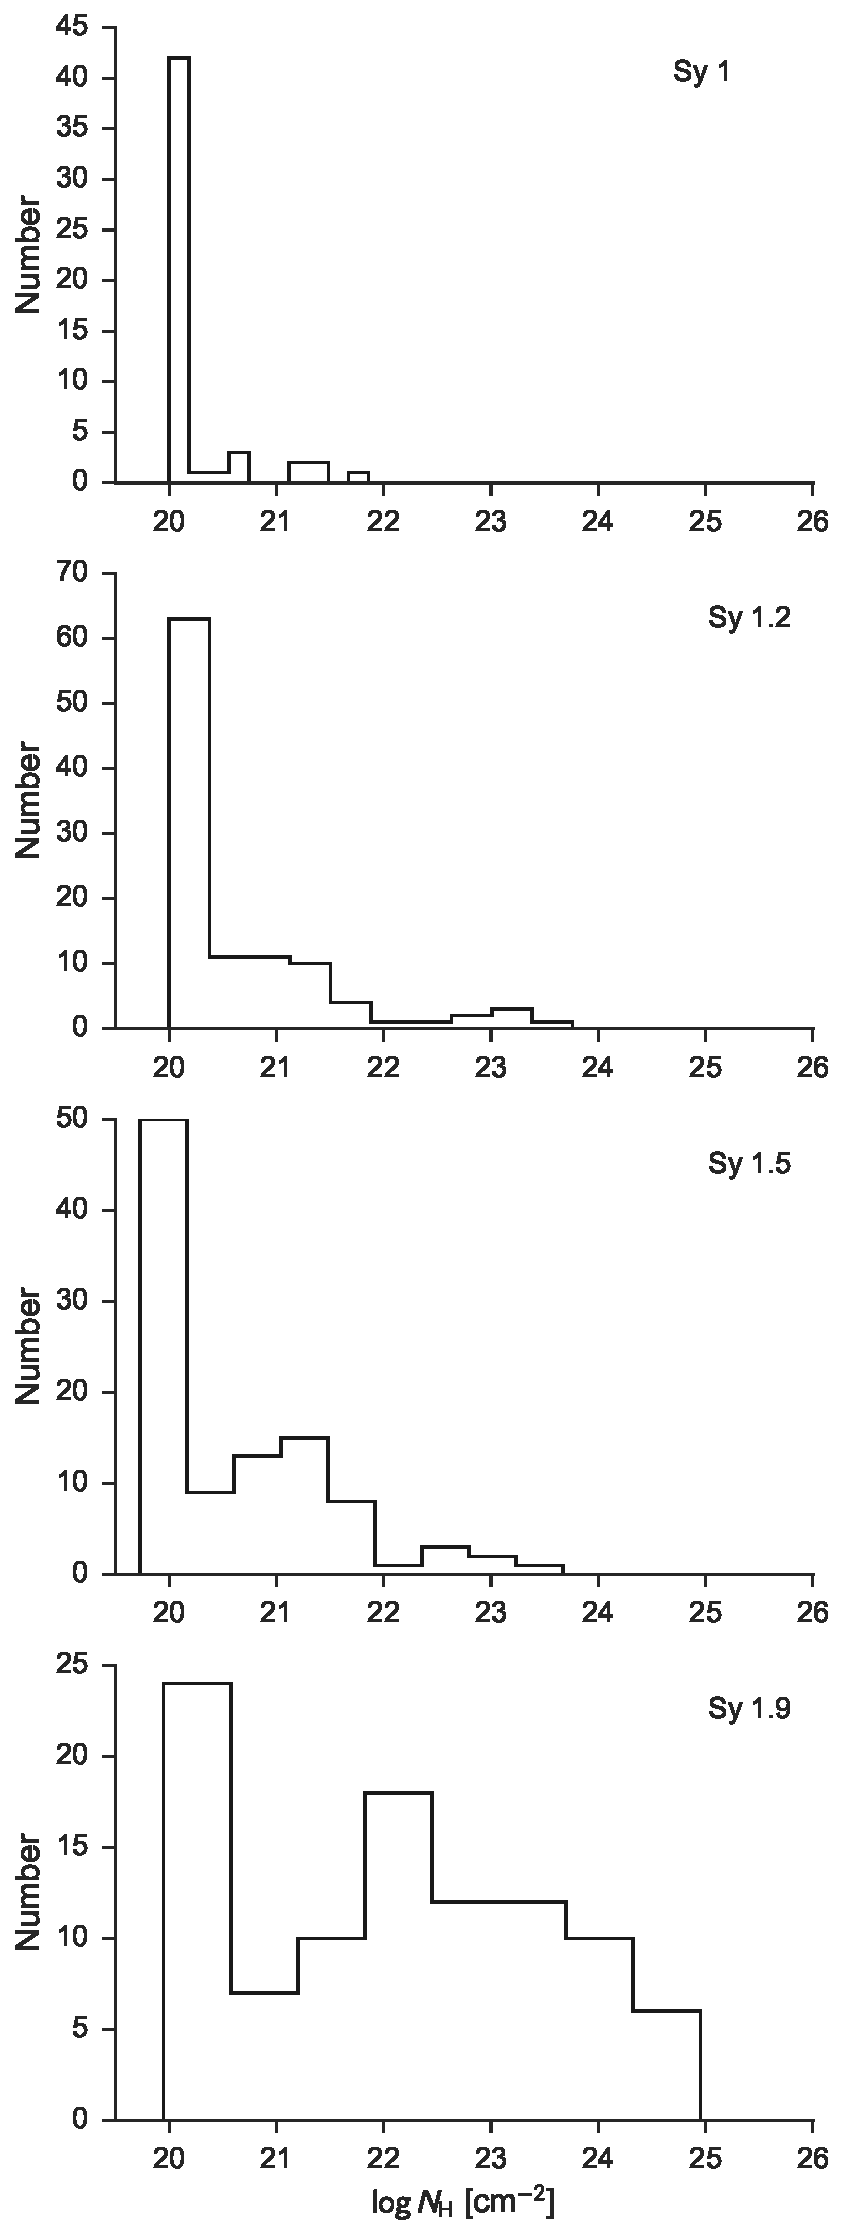
\includegraphics[width=\columnwidth]{../figures/nh_hists_only_sy1.pdf}
\caption{\label{fig:nh_dist}\nh{} distribution for Sy 1s, 1.2s, 1.5s and 1.9s in our full sample.}
\end{figure}
%%%%%%%%%%%%%%%%%%%%%%%%%%%%%%%%%%%%%%%%%%%%%%%%%%%%%%%%%%% 

\subsection{Broad \halpha{} vs. X-ray Luminosity}
Our determination of the optical obscuration occurring in Sy 1.9s hinges on a direct relationship between the broad \halpha{} luminosity and the AGN luminosity. We assume the intrinsic X-ray luminosity is an accurate tracer of the bolometric AGN luminosity as has been shown in previous studies \citep[e.g.][]{Winter:2012yq}. In Fig.~\ref{fig:brha_xray}, we show the correlation between the broad \halpha{} and intrinsic X-ray luminosities for Sy 1-1.2s as blue dots. The correlation is highly significant with a Pearson correlation coefficient of 0.85 and p-value of $10^{-35}$. 

Fig.~\ref{fig:brha_xray} indicates our assumption that the broad \halpha{} luminosity closely follows the AGN luminosity is correct. Therefore, we can use the intrinsic X-ray luminosity to predict the non-obscured broad \halpha{} luminosity and compare it with the observed broad \halpha{} luminosity as a measure of the optical obscuration towards the BLR. We fit a simple line using linear least squares between the broad \halpha{} luminosity and intrinsic X-ray luminosity finding the following relation:

\begin{equation}\label{eq:brha-xray}
\log\,L_{\rm H\alpha, broad} = 1.06\log\,L_{14-150\,keV} - 4.32
\end{equation}

We plot Equation~\ref{eq:brha-xray} in Fig.~\ref{fig:brha_xray} as a blue line along with shading to indicate our measured 0.4 dex scatter. As red squares we show our Sy 1.9 sample with black circles indicating the X-ray absorbed objects. Sy 1.9s lie systematically below the relationship defined by the Sy 1-1.2s and well outside the estimated scatter. The black dotted line indicates a reduction factor of 100 in the broad \halpha{} luminosity and highlights roughly the maximum decrease we observe for Sy 1.9s. We also plot Sy 1.5s as black diamonds to show that while they were not included in our calculation of the best fit, Sy 1.5s also lie along the line and within the scatter.

If we assume that the reduction in broad \halpha{} luminosity is completely due to obscuration, we can calculate the visual extinction, $A_{\rm V}$, given an extinction law. For this work, we use the empirically determined extinction law from \citet{Wild:2011aa} that was also used in our previous study investigating BLR obscuration \citep{Schnorr-Muller:2016qy}.  The maximum luminosity decrease we observe then corresponds to a maximum $A_{\rm V}\sim6$ mag. 

If we then also assume a Galactic \nh/$A_{\rm V}$ ratio of $1.87\times10^{21}$ cm$^{-2}$ \citep{Draine:2011zr}, we expect for our Sy 1.9 sample a maximum \nh{}$\sim10^{22}$ cm$^{-2}$, the cutoff we used for our definition of X-ray absorbed. Therefore, based on the optical obscuration towards the BLR, we would expect virtually all of our Sy 1.9s to be X-ray unabsorbed. Instead, Fig.~\ref{fig:nh_dist} shows that over half of the Sy 1.9s have \nh{} values above 10$^{22}$ cm$^{-2}$ meaning along our lines of sight towards a significant fraction of Sy 1.9s, there is either more or different gas and dust hiding the central X-ray source than there is in front of the BLR.

%%%%%%%%%%%%%%%%%%%FIGURE: Broad Halpha vs. X-ray%%%%%%%%%%%%%%%%%%%%%%%
\begin{figure*}
\centering
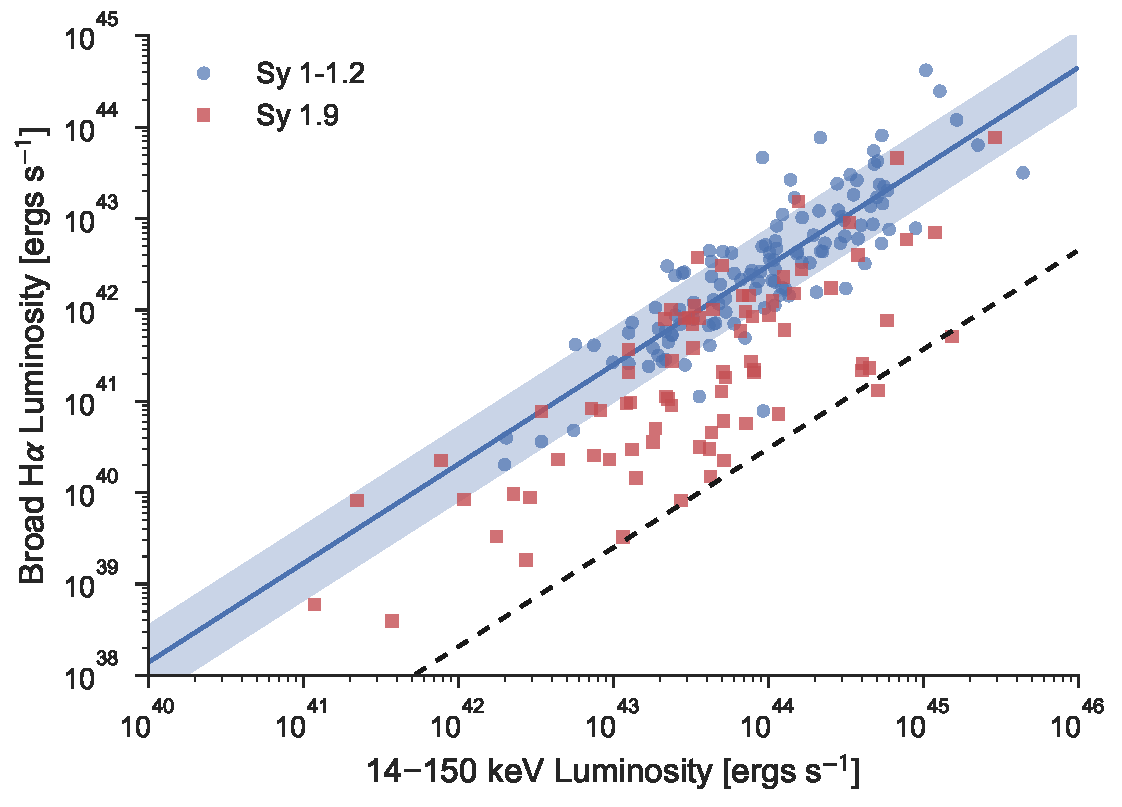
\includegraphics[width=0.8\textwidth]{../figures/halpha_vs_xray_with2dexLine.pdf}
\caption{\label{fig:brha_xray} The relationship between intrinsic X-ray (14--150 keV) luminosity and observed broad \halpha{} luminosity for BASS selected Sy 1--1.9s. Blue dots correspond to Sy 1--1.2s which were used to measure the best-fit line (solid blue line) and scatter (blue shaded region) between the X-ray emission and broad \halpha{} emission. Black diamonds show the Sy 1.5s while red squares plot the Sy 1.9s. X-ray absorbed sources (\nh{} $>10^{22}$ cm$^{-2}$) are encircled. The black dashed line shows our chosen threshold for optically obscured sources which are $>2\sigma$ below the measured best-fit line while the black dotted line shows approximately the maximum reduction we observe in broad \halpha{} of 2 dex.}
\end{figure*}
%%%%%%%%%%%%%%%%%%%%%%%%%%%%%%%%%%%%%%%%%%%%%%%%%%%%%%%%%%

%%%%%%%%%%%%%%%%%%FIGURE: NH distribution for Sy 1.9 obscured and unobscured%%%%%%%%%%%%%
\begin{figure}
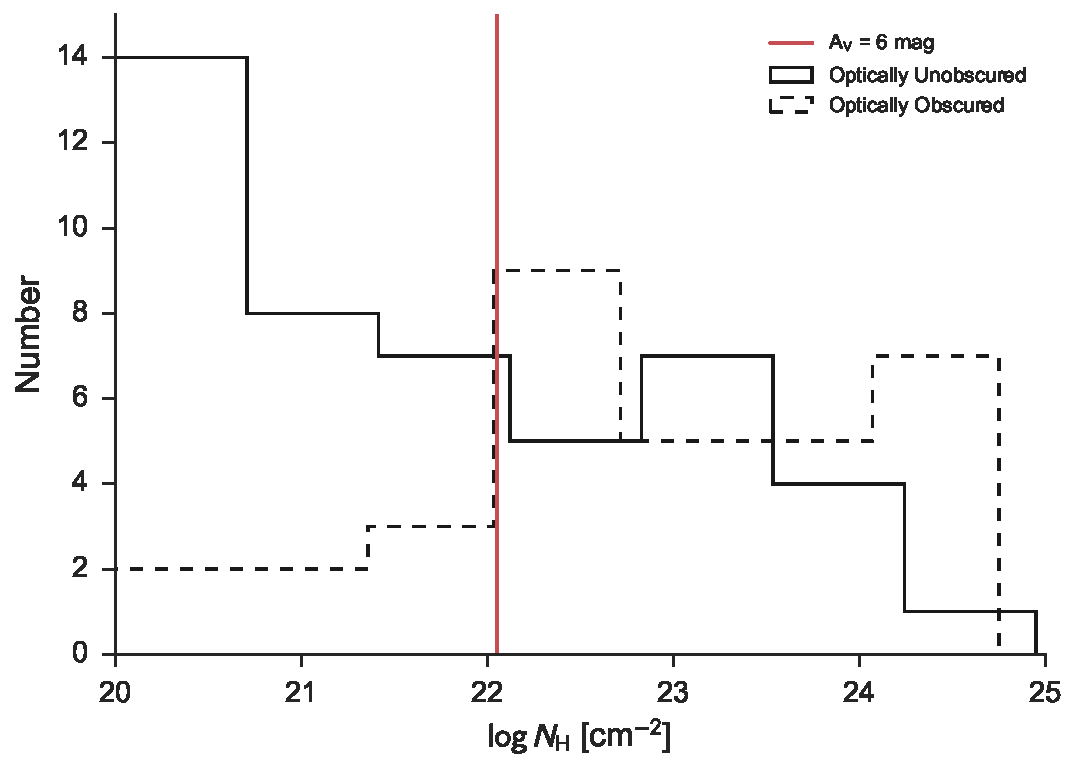
\includegraphics[width=\columnwidth]{../figures/nh_hists_sy1_9_split_optical_obscuration.pdf}
\caption{\label{fig:nh_dist_sy1_9} Distribution of \nh{} for optically obscured (dashed line) and unobscured Sy 1.9s. Optically obscured sources are defined as those that lie at least 2$\sigma$ below the X-ray-to-broad \halpha{} relationship shown in Fig.~\ref{fig:brha_xray}. The red solid line indicates the maximum \nh{} expected given the maximum $A_{\rm{V}}\sim6$ mag observed (dotted line in Fig.~\ref{fig:brha_xray}. }
\end{figure}
%%%%%%%%%%%%%%%%%%%%%%%%%%%%%%%%%%%%%%%%%%%%%%%%%%%%%%%%%%

However, while the column densities toward the BLR and X-ray corona seem to be discrepant for Sy 1.9s, the occurrence of optical obscuration and X-ray absorption do seem to be related in a way that most of the Sy 1.9s that appear to be optically obscured also show X-ray absorption. To highlight this, we split the Sy 1.9s based on their location in Fig~\ref{fig:brha_xray}. ``Optically obscured'' sources are at least 2$\sigma$ (0.8 dex; dashed line) below the Sy 1-1.2 relationship while the rest are ``optically unobscured.''   In Fig.~\ref{fig:nh_dist_sy1_9} we show the X-ray derived \nh{} distributions for each of these subsamples with optically unobscured sources plotted as a solid line and optically obscured sources plotted as a dashed line. Further, in Table~\ref{tab:sy1_9_numbers}, we report the absolute numbers within the four categories for optical obscuration and X-ray absorption. 

Below $N_{\rm H} = 10^{22}$ cm$^{-2}$, the majority of Sy 1.9s (17/23) are optically unobscured while above this threshold, many (22/38) are optically obscured.  This indicates that the obscuring structures towards both the X-ray emitting region, presumably very near to the SMBH, and the BLR, farther out, are related, just not at the same absolute level. We show, as a red line in Fig.~\ref{fig:brha_xray},  the maximum amount of \nh{} expected based on the maximum optical obscuration we observe ($A_{\rm V} \sim 6$ mag). Even though a large fraction of optically obscured Sy 1.9s are also X-ray absorbed (79\%; see Table~\ref{tab:sy1_9_numbers}), the level of X-ray absorption is much higher. In fact, given a maximum $A_{\rm V}$ of 6 mag, we would expect virtually no Sy 1.9s with \nh{}$>10^{22}$ cm$^{-2}$ just as we see for the Sy 1-1.5s.

\begin{deluxetable}{lccc}
\tablecaption{Optical Obscuration and X-ray Absorption in Sy 1.9s\label{tab:sy1_9_numbers}}
\tablehead{%
\colhead{} & \colhead{X-ray Unabsorbed} & \colhead{X-ray Absorbed} & \colhead{Total}
}
\startdata
Optically Unobscured & 17 & 16 & 33 \\
Optically Obscured & 6 & 21 & 27 \\
Total & 23 & 38 & 61 \\
\enddata
\end{deluxetable}

\section{Discussion}\label{sec:discuss}

%%%%%%%%%%%%%%%%%%FIGURE: Fraction X-ray Absorbed vs. X-ray luminosity%%%%%%%%%%%%%
\begin{figure}
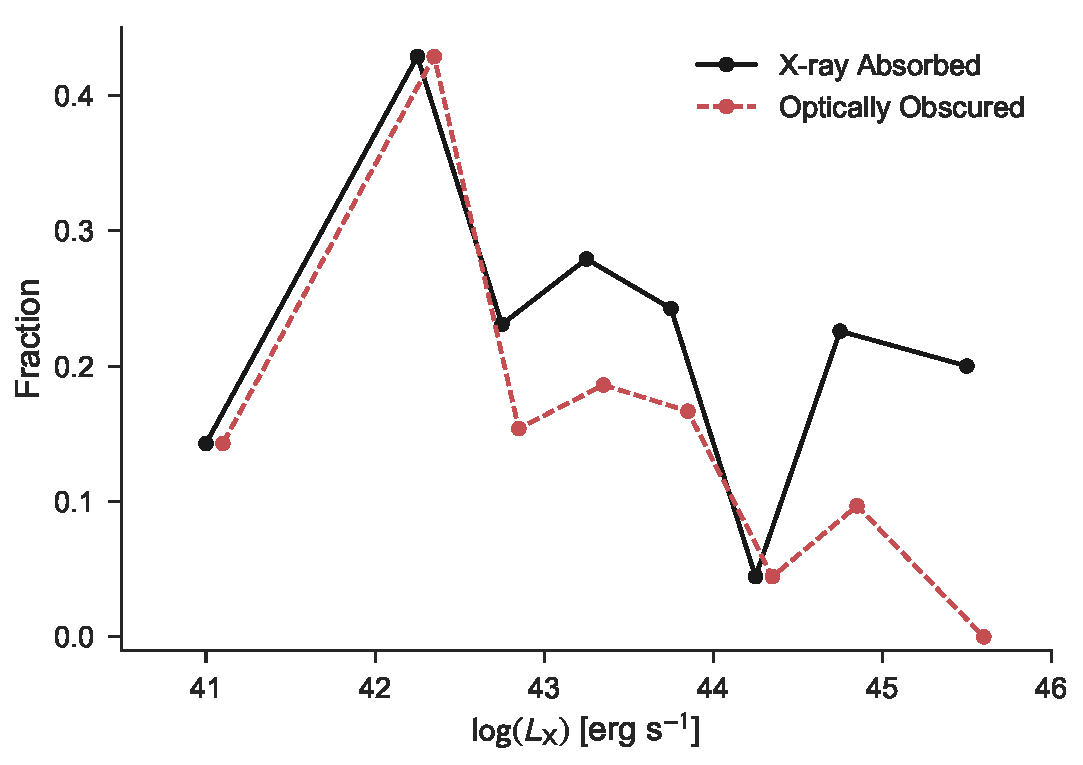
\includegraphics[width=\columnwidth]{../figures/frac_blagn_xray_abs_and_opt_obs_vs_lx.pdf}
\caption{\label{fig:frac_xabs} The fraction of X-ray absorbed (black dots and solid line) and optically obscured (red dots and dashed line) Sy 1-1.9s as a function of intrinsic X-ray luminosity. The optically obscured bins have been shifted by +0.1 dex to avoid overlap. There is a clear drop in the number of optically obscured sources towards high AGN luminosity while the X-ray number of X-ray absorbed sources is relatively flat.}
\end{figure}
%%%%%%%%%%%%%%%%%%%%%%%%%%%%%%%%%%%%%%%%%%%%%%%%%%%%%%%%%%



\section{Conclusions}\label{sec:conclude}

\acknowledgments
\facilities{}
\software{%
	\textsl{astropy} \citep{Astropy:2013ek},
	\textsl{pandas} \citep{McKinney:2010em},
	\textsl{matplotlib} \citep{Hunter:2007},
	\textsl{numpy} \citep{vanderWalt:2011we},
	\textsl{scipy} \citep{Jones:2001ch}
}
	
\bibliographystyle{aasjournal}
\bibliography{/Users/ttshimiz/Dropbox/Research/my_bib}

\end{document}